\section{Hardware}
\label{chptr:hardware}
In diesem Kapitel wird die Hardware der Steuerung im Detail erläutert. Es wird genauer auf die technischen Details der verwendeten Komponente eingegangen und auf ihre Aufgabe in der Steuerung.

\subsection{Raspberry PI}
Dieser wurde ausgewählt, weil dieser mit sämtlichen industriellen Schnittstellen kompatibel ist. Darunter auch mit der SPS, die im nächsten Kapitel beschrieben ist. Dieser ist die Hauptkomponente und dient als Zentrale für die Evaluierung sämtlicher Berechnungen und gibt die Befehle an den TEC-Treiber und an den Diodetreiber bzw. SPS und steuert die Digitalanzeige. Der Rechner ist direkt auf der SPS montierbar und benötigt somit weniger Platz im Gehäuse der Steuerung. Die Kommunikation des Rechners zur SPS erfolgt über ein Flachbandkabel. Worüber mit Pythonprogrammen direkt Ein- und Ausgänge auf der SPS angesteuert werden können. Somit ist es möglich etliche weitere Komponente anzuschliessen und zu steuern. So auch der Diodentreiber, der im Kapitel \ref{chptr:_diodentreiber} näher beschrieben wird. Der TEC-Treiber kommuniziert direkt über die USB2.0-Schnittstelle auf dem Rechner und muss nicht über die SPS gesteuert werden.\\
Das Betriebssystem des Raspberry PI ist ein Derivat des Linux Betriebssystems. Mit einem Image speziell für einen Raspberry PI, können standardmässig Programme zum Programmieren von Pythonskripten und die Pythoninstallation mit installiert werden. Die weiter oben beschriebenen Standardbibliotheken sind ebenfalls in der Basisinstallation der Pythondistribution enthalten. Die zusätzlichen Bibliotheken von Drittanbietern mussten jedoch noch nachträglich installiert werden, diese sind im Anhang teilweise beschrieben.

\begin{figure}[H]
    \centering
    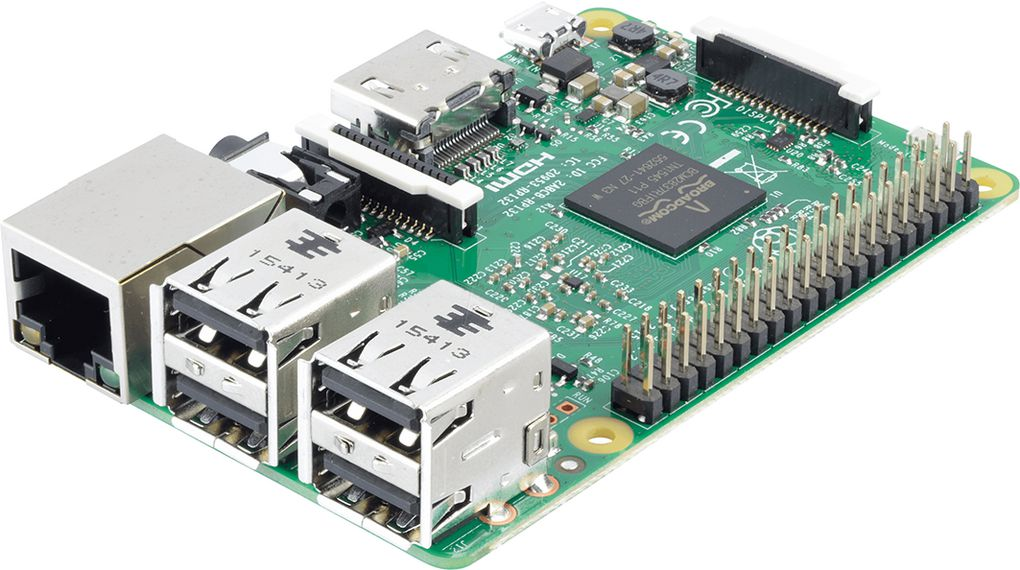
\includegraphics[scale=0.25]{98_images/raspberry_pi_version_3_b.jpg}
    \caption{Ein \textit{Raspberry PI}-Einplatinenrechner der Version  3B+. [15]}
    \label{fig:raspberry_pi_3b+}
\end{figure}

\subsection{SPS - PiXtend}
Die Ein- und Ausgänge, die der Raspberry PI steuert sind mit einer SPS des Herstellers PiXtend L 2.1 realisiert. Dies ist eine Steuerung, auf welche der Rechner direkt aufgeschraubt werden kann. Alle benötigten Ein- und Ausgänge für die Steuerung des Pumpdiodentreibers befinden sich direkt auf der Platine. Von grosser Wichtigkeit sind die analogen Ein- und Ausgänge um den Ausgangsstrom des Treibers zu steuern bzw. den Ausgangsstrom zurück in die SPS zu geben, um später die optische Leistung zu evaluieren. Die Fähigkeit analoge Signale zu verarbeiten, war der Grund, diese Steuerung auszuwählen.

\begin{figure}[H]
    \centering
    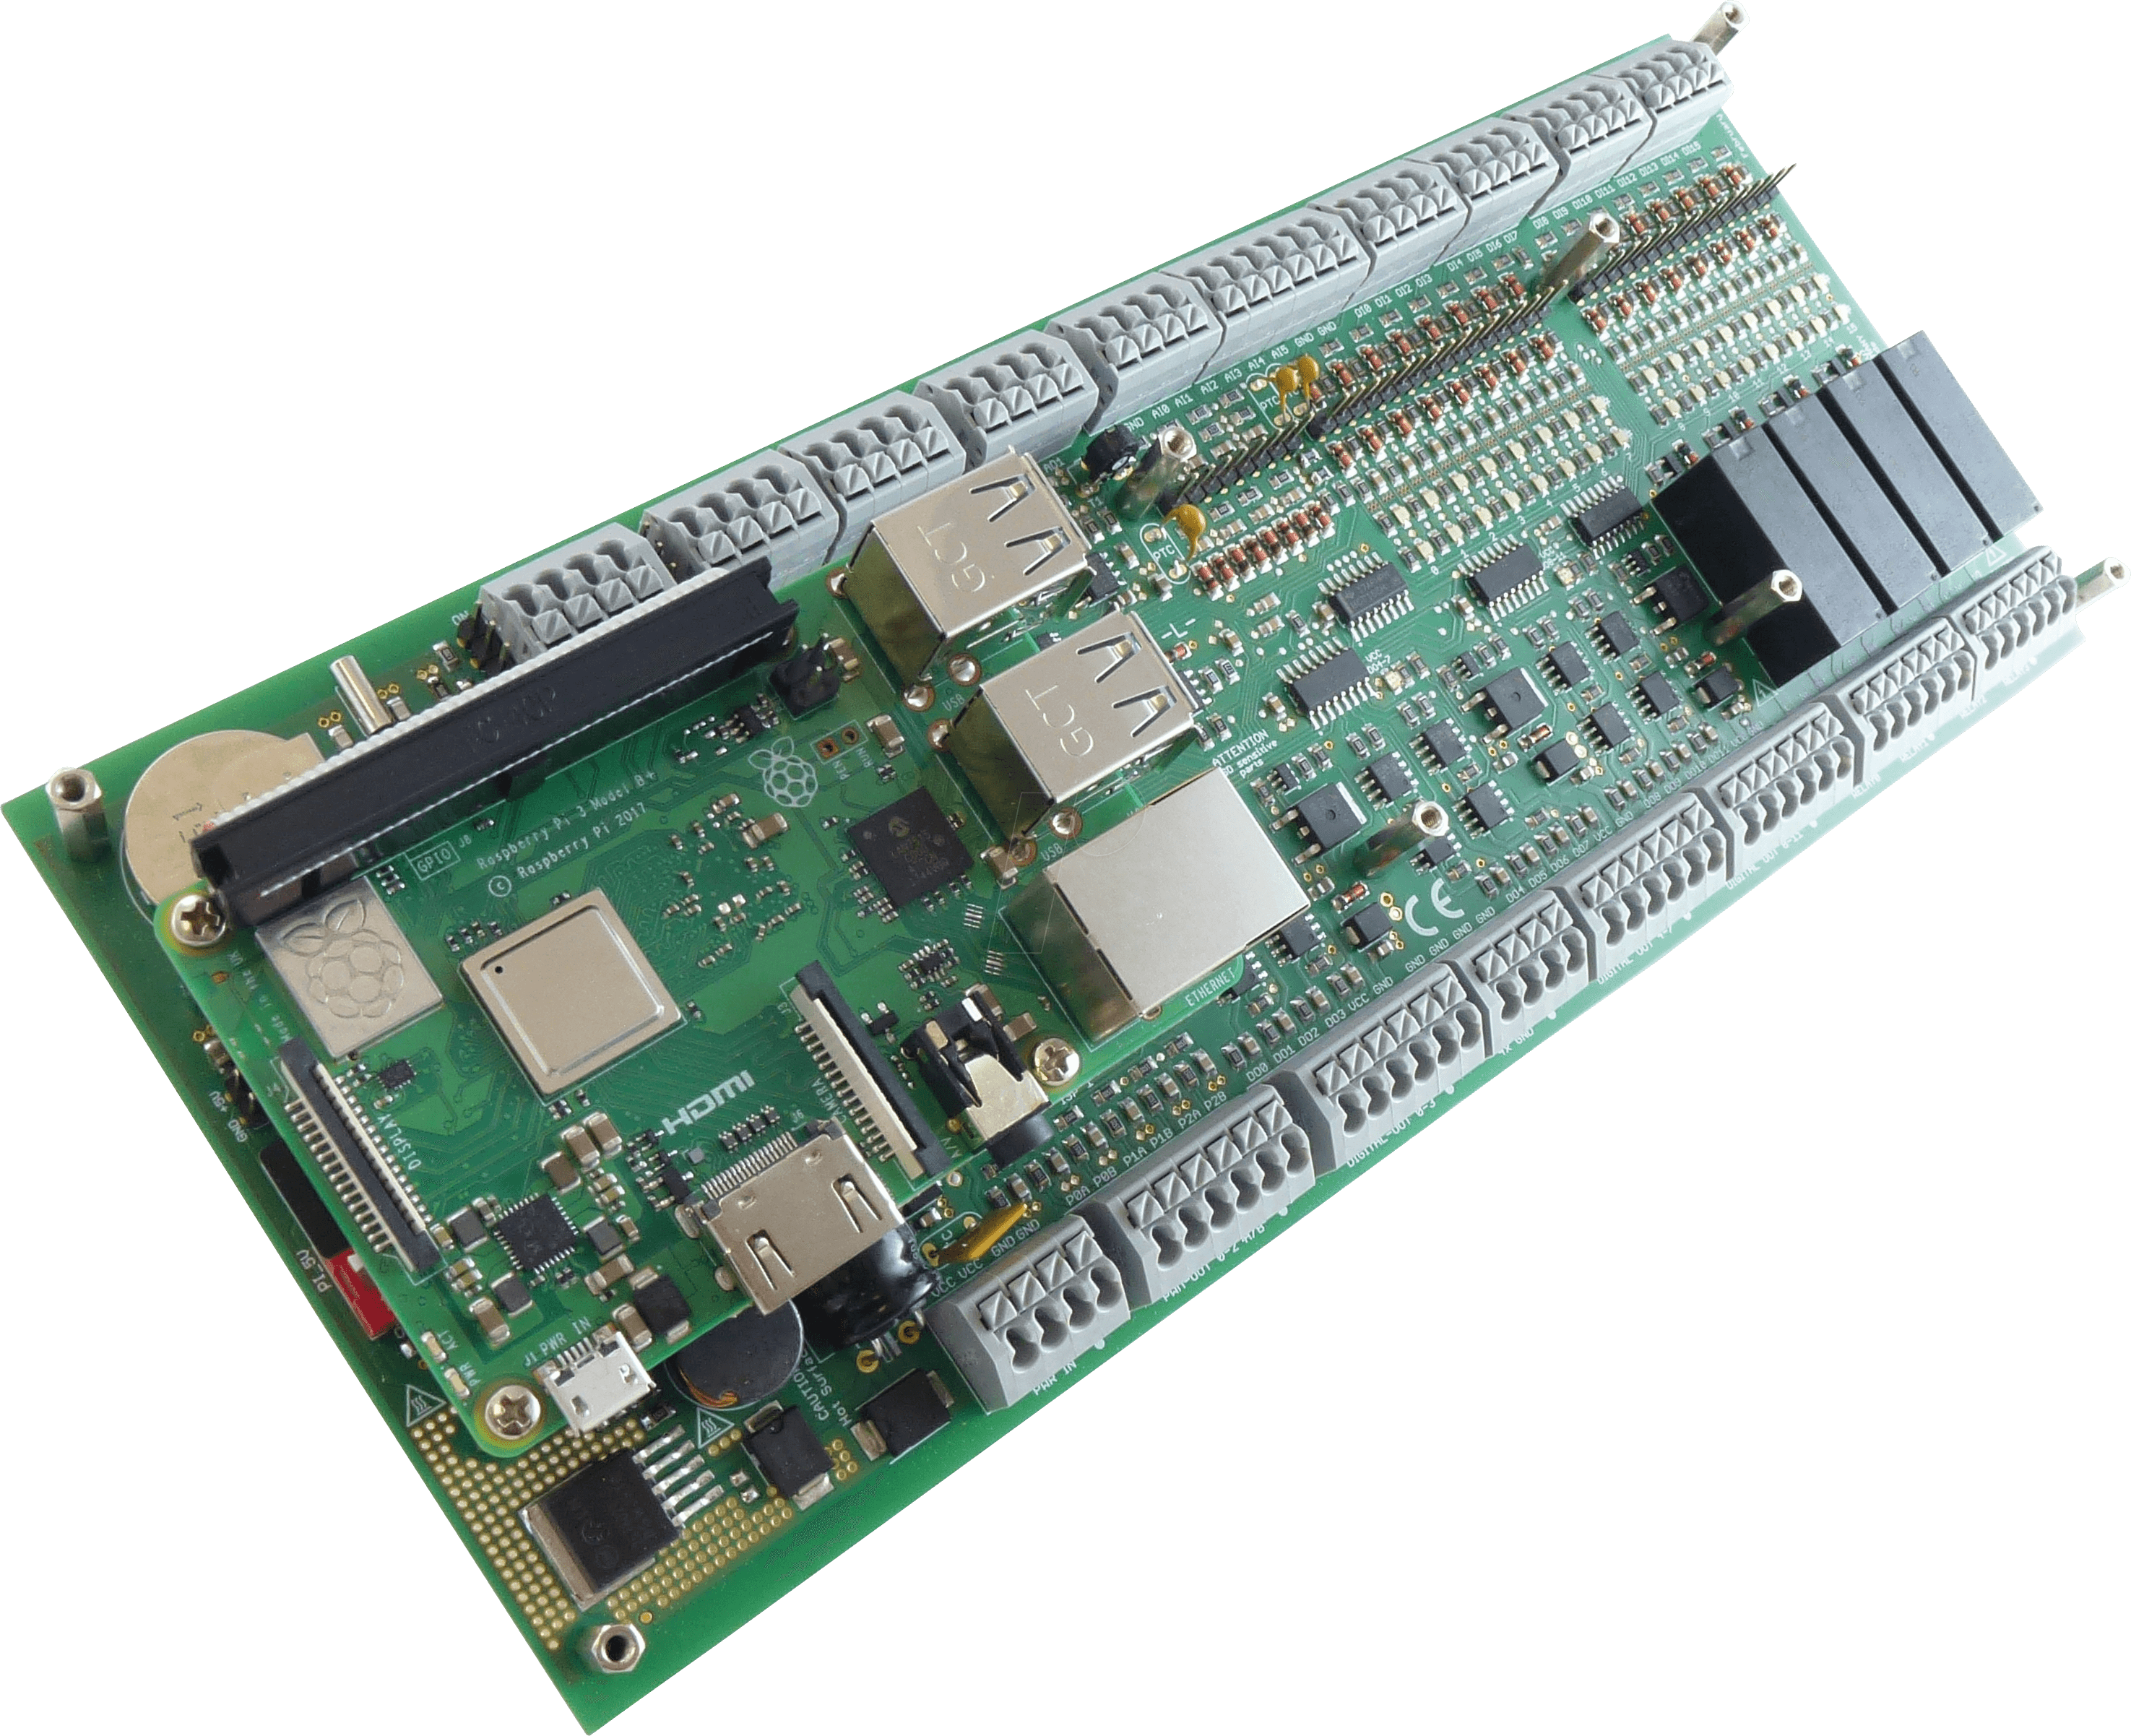
\includegraphics[scale=0.08]{98_images/pixtend_l_basic.png}
    \caption{Die \textit{SPS PiXtend L V2.1} des Herstellers \textit{Kontron}. Der Raspberry PI ist auf der linken Seite auf der SPS montiert ersichtlich. [18]}
    \label{fig:sps_pixtend_hw}
\end{figure}

\subsection{Thermoelektrischer Kühler - TEC}
Die beiden verwendeten TECs werden unter der Pumpdiode bzw. der Halterung des Alexandritkristalls montiert. Sie dienen dazu die Wärme vom Kristall und von der Pumpdiode abzuleiten. Dazu wird jeweils die kühle Seite dem zu kühlenden Objekt zugewandt, ersichtlich ist dies in der Abb. \ref{fig:_tec_cr_hw}. Die Wärme der warmen Seite wird mit einer Wasser- oder Luftkühlung aus dem System geführt. Die Temperatur an den zu kühlenden Objekten wird mit Thermistoren, gemessen. So kann über ein Regelkreis mit dem TEC-Kontroller die gewünschte Temperatur eingestellt werden. Die Thermistoren sollen so nah wie möglich an dem zu messenden Objekt platziert werden. Auf der Abb. \ref{fig:_thermistor_cr} ist die Position für den Thermistor des Kristalls angezeigt. Auf dieser Seite ist der Steg für die Bohrung in die Halterung stark genug, um die Steifigkeit der Halterung nicht massiv zu verringern, auch wird der Laserstrahl, der links und rechts an der Halterung vorbei muss nicht behindert.

\begin{figure}[H]
    \centering
    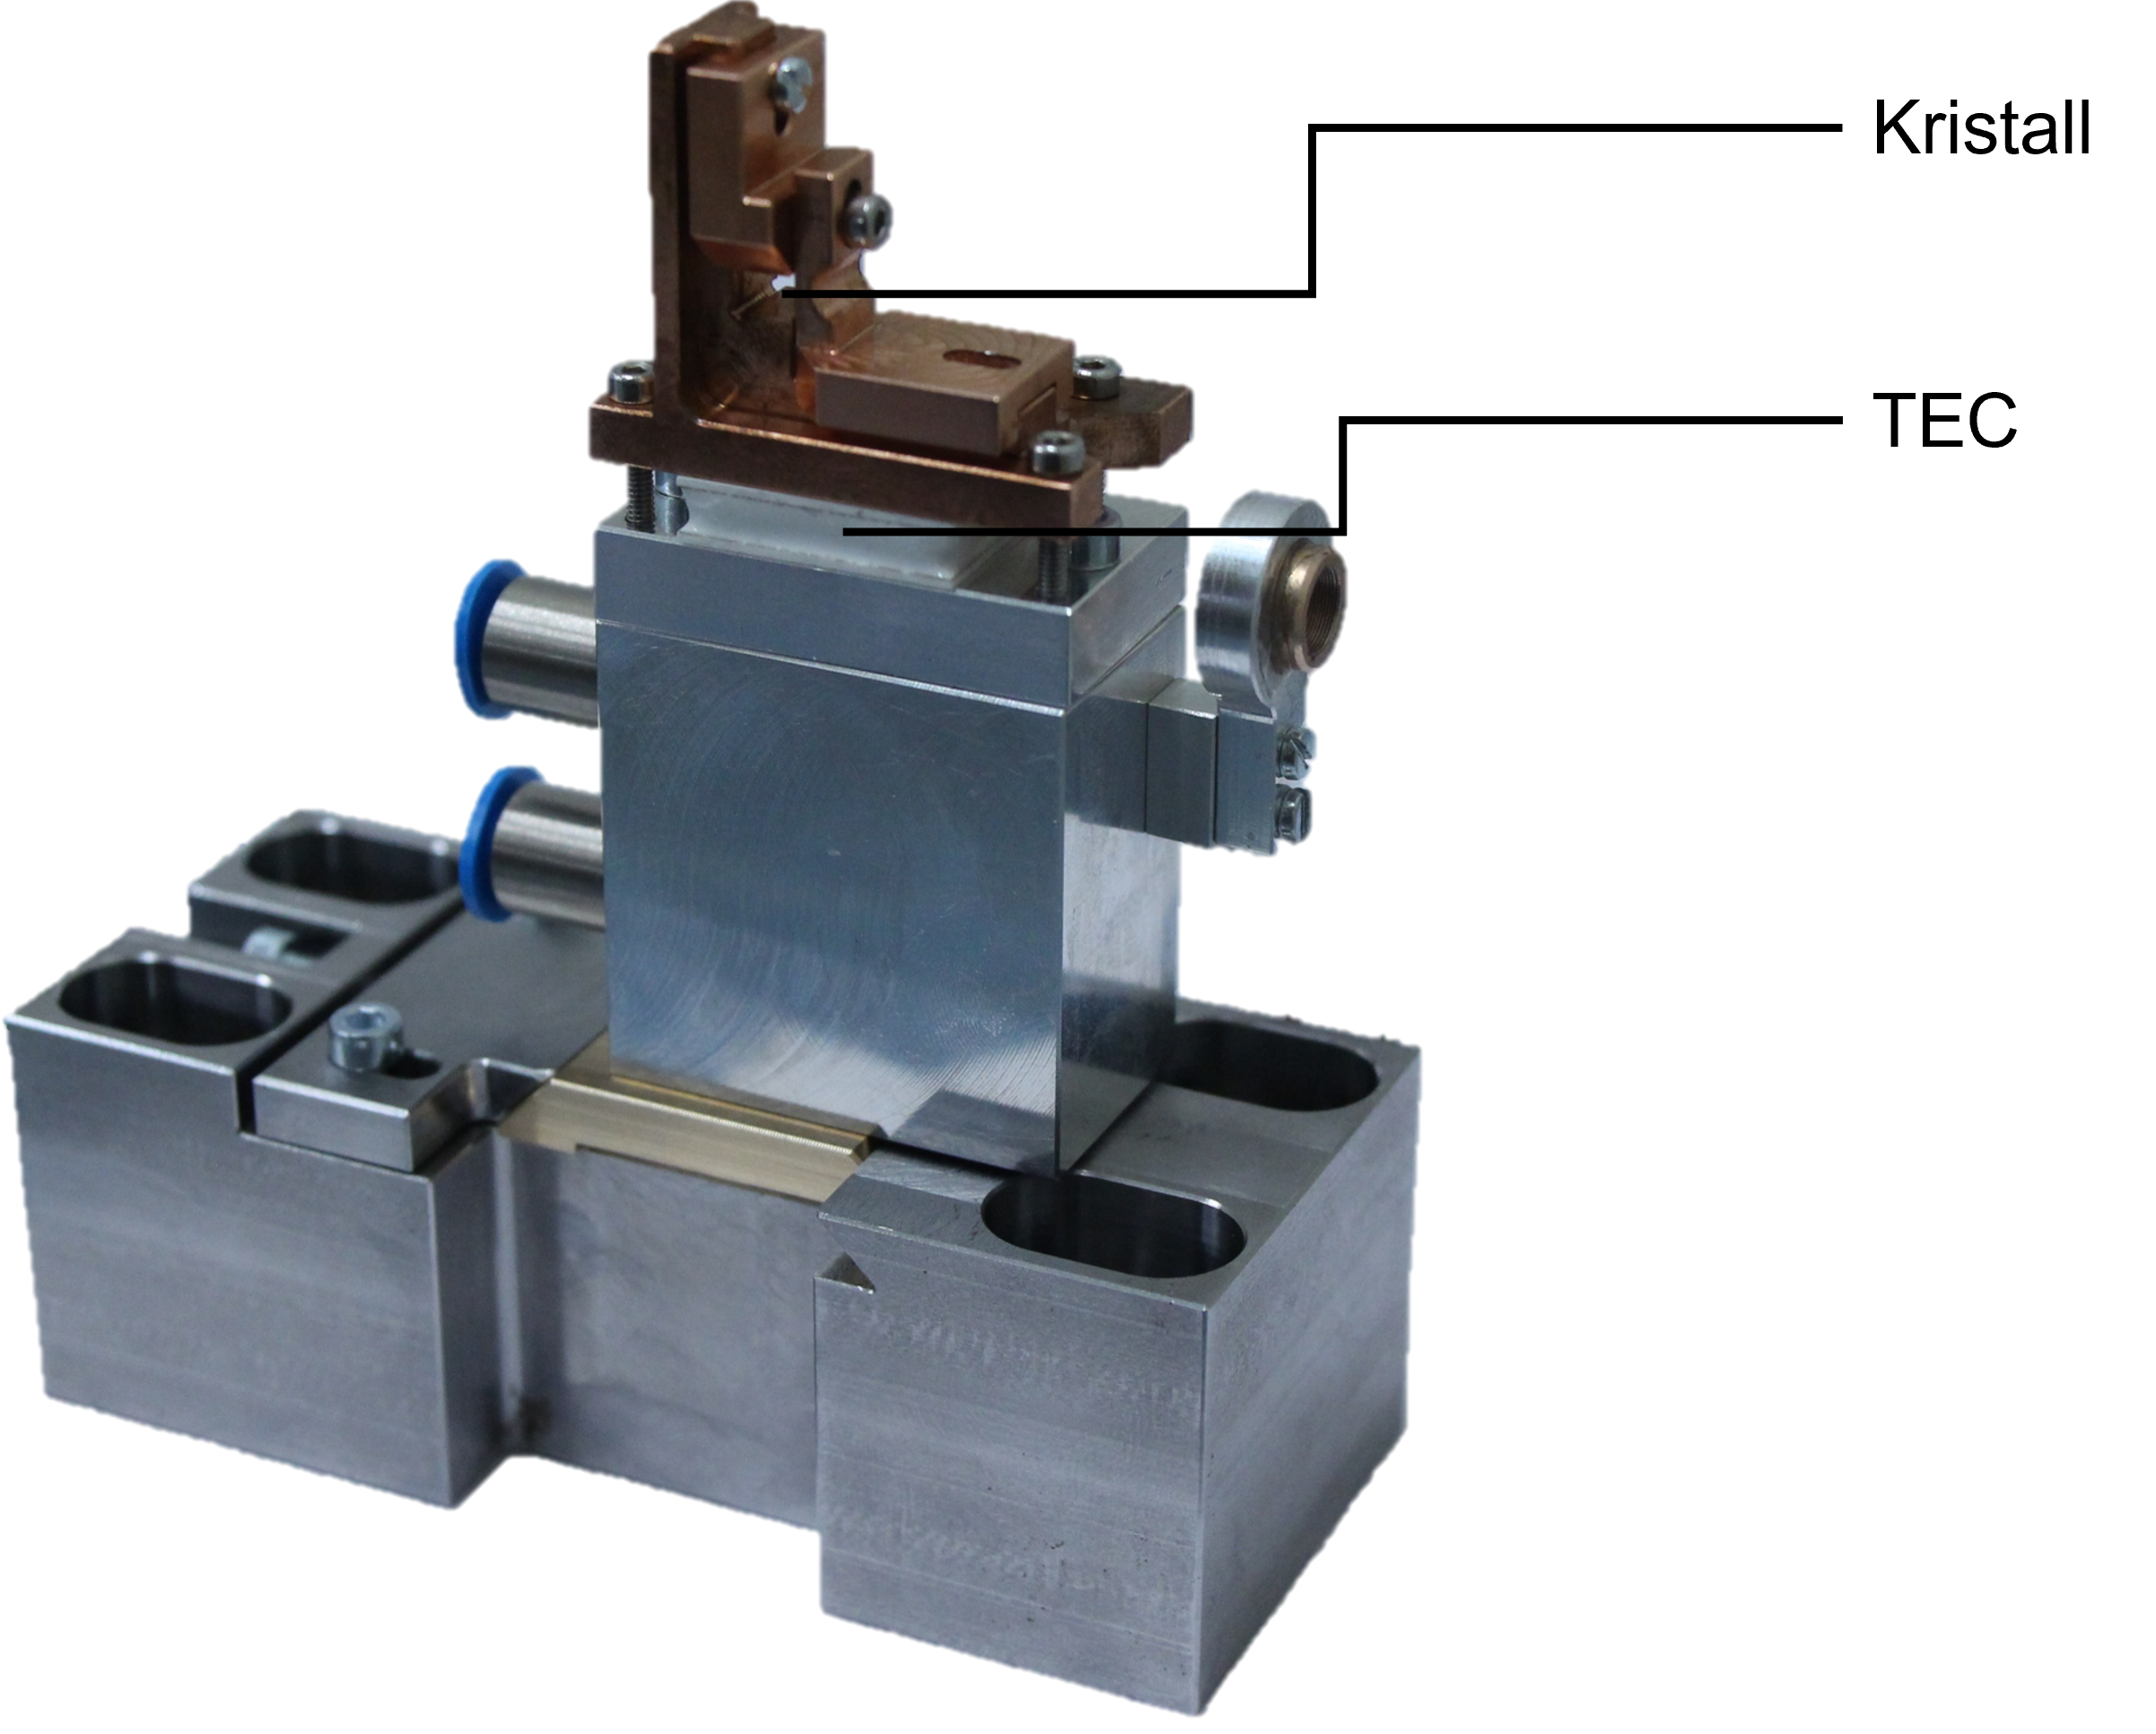
\includegraphics[scale=0.5]{98_images/real_front_desc.png}
    \caption{In der Abbildung ist der TEC in der Kristallhalterung gezeigt. [20]}
    \label{fig:_tec_cr_hw}
\end{figure}

\begin{figure}[H]
    \centering
    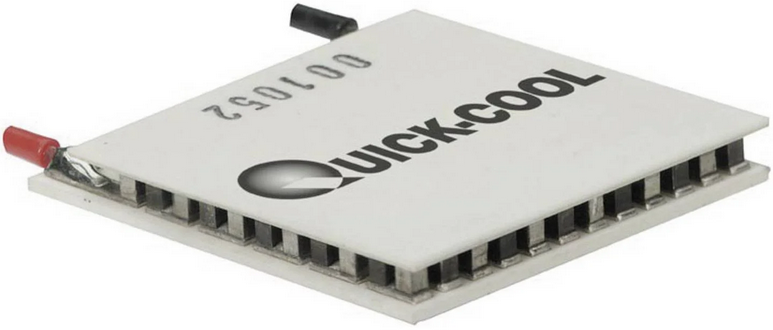
\includegraphics[scale=0.5]{98_images/peltier_modul.PNG}
    \caption{Abgebildet ist der thermoelektrische Kühler für die Diode. [8]}
    \label{fig:tec_di_hw}
\end{figure}

\subsection{TEC-Treiber}
\label{label_tec_treiber}
Aus dem Grund, dass zwei TECs gesteuert werden sollen, wurde ein zwei-kanaliger TEC-Treiber des Herstellers Meerstetter Engineering verwendet, dieser erfüllt alle benötigten Voraussetzungen. Obwohl die Leistung von diesem zu hoch ist, wurde dieser ausgewählt weil er bereits im Institut vorhanden gewesen ist. Die Lieferzeiten hätten unter Umständen die Dauer der vorliegenden Arbeit ausgeschöpft.\\
Auf der Softwareseite sind die Signale, hier die Temperaturen, eindeutig identifizierbar, was mit zwei ein-kanaligen Treibern nicht ohne Weiteres möglich gewesen wäre. Die Informationen werden über einen BUS an den zentralen Rechner (Raspberry PI) gesendet und da weiter verarbeitet bzw. auf der Digitalanzeige angezeigt.
Die Temperaturen der TECs werden über ein TEC-Kontroller mit einem PID-Regler eingestellt, wie weiter oben erwähnt. Zusätzlich ist der Kontroller von Meerstetter Engineering in der Lage diese PID-Parameter automatisch zu finden und müssen nicht gesucht oder gar separat berechnet werden. Dies wurde auf dem Testaufbau realisiert, wo die Voraussetzungen für den Betrieb der Komponenten am nächsten an der künftigen Laseraufbau waren. [19]\\
Die Energieversorgung der Steuerung kann lediglich eine maximale Leistung abgeben. Damit die Zuverlässigkeit der Steuerung, muss der Strom deshalb begrenzt werden. Die Begrenzung des Stromes ist integraler Bestandteil des Kontrollers und kann direkt in der Software des TEC-Kontrollers vorgenommen werden und muss nicht separat Programmiert werden.\\
Die Leistung reicht aus, um die Diode bis zu einer optischen Leistung von ca. 4.5W mit einer Kühlwassertemperatur von ca. 23.5°C zu kühlen. Über diesen Temperaturen kann die von der Pumpdiode abgegebene Wärme nicht mehr dissipiert werden. Folglich staut sich im Sockel die Wärme der Pumpdiode bzw. der Kristallhalterung. Der Regler kann nicht mehr regeln und die Temperaturen steigen kontinuierlich. Die Wasserkühlung muss deshalb mit niedrigeren Temperaturen als diese 23.5°C betrieben werden. Dazu ist auch eine Begrenzung der Temperaturen der Pumpdiode vorzusehen, auch dies konnte in der Software des Kontrollers vorgenommen werden. Es stellt sicher, dass die Temperatur des Kristalls bzw. der Pumpdiode eine gewisse Höhe nicht überschreiten kann. Dies ist notwendig, weil bei zu hohen Temperaturen die Pumpdiode in Mitleidenschaft gezogen werden könnte. In der Tabelle \ref{tab:_tec_a_limit} sind die Einstellungen für die Ströme beider TECs ersichtlich gleich darunter, in der  Abb. \ref{fig:_tec_treiber_hw} ist der TEC-Kontroller von Meerstetter abgebildet.

\begin{figure}[H]
    \centering
    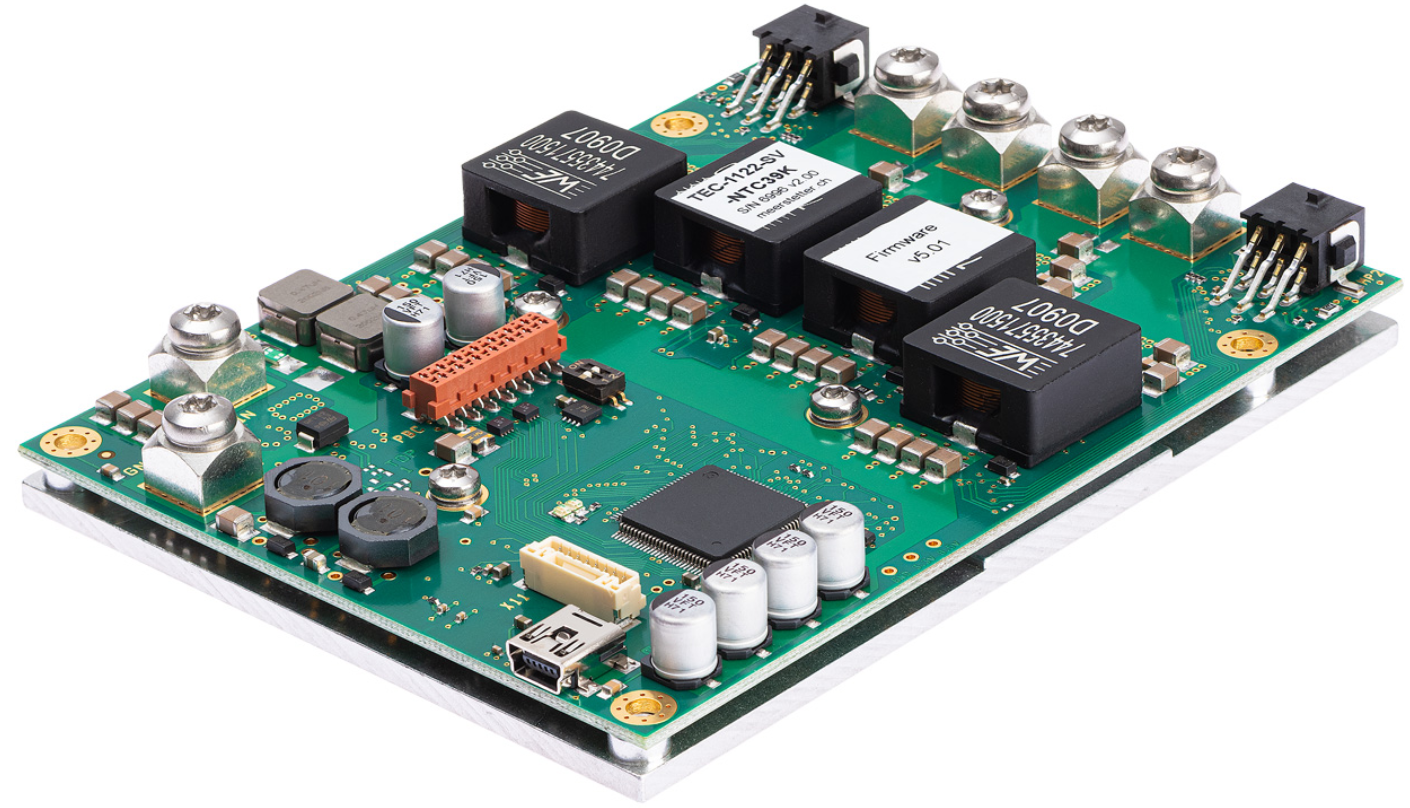
\includegraphics[scale=0.2]{98_images/tec_controller_real_isometry_meerstetter.PNG}
    \caption{Ein zwei-kanaliger TEC-Treiber vom Hersteller Meerstetter Engineering. [19]}
    \label{fig:_tec_treiber_hw}
\end{figure}

\begin{table}[H]
    \centering
    \begin{tabular}{l|l|l}
         \textbf{TECs}& \textbf{Max. Strom}&    \textbf{Max. Temperatur} \\
         \hline
         Diode&         1.5A&                   15°C - 35°C [1]\\
         Kristall&      0.75A&                  $-$
    \end{tabular}
    \caption{Begrenzung der Ströme für die TECs des Kristalls und der Diode}
    \label{tab:_tec_a_limit}
\end{table}

\subsection{Pumpdiodentreiber}
\label{chptr:_diodentreiber}
Der Pumpdiodentreiber oder auch Diodentreiber wurde vom Hersteller \textit{Opt Lasers} bezogen. Auf der Abb. \ref{fig:diodentreiber_hw} ist der Diodentreiber abgebildet. Die Pumpdiode wird mit 30V und bis zu etwa 0.5A betrieben, benötigt dementsprechend eine Eingangsleistung von mindestens 15W. [1] Der Diodentreiber verfügt über eine Spannung zwischen 5V-35V und kann mit bis zu 1.5A gespeisen werden. Um die Laserdiode jedoch vor der Zerstörung zu bewahren, wurde die Stromstärke auf 0.8A beschränkt. [1] Dies wurde physisch direkt auf dem Bauteil beim Potentiometer (Abb. \ref{fig:_diodentreiber_hw} in blau) vorgenommen, andererseits in der Software im Raspberry PI hinterlegt. Auf den Aufbau der Software des Diodentreibers wird im Kapitel \ref{chptr:software} noch genauer eingegangen.\\
Ergänzend bleibt der Diodentreiber Stromlos, sollte ein Notaus-Taster betätigt werden und startet nicht wieder sollte die Steuerung wieder eingeschaltet werden. Diese Funktion ist ein integraler Bestandteil des Diodentreibers.

\begin{figure}[H]
    \centering
    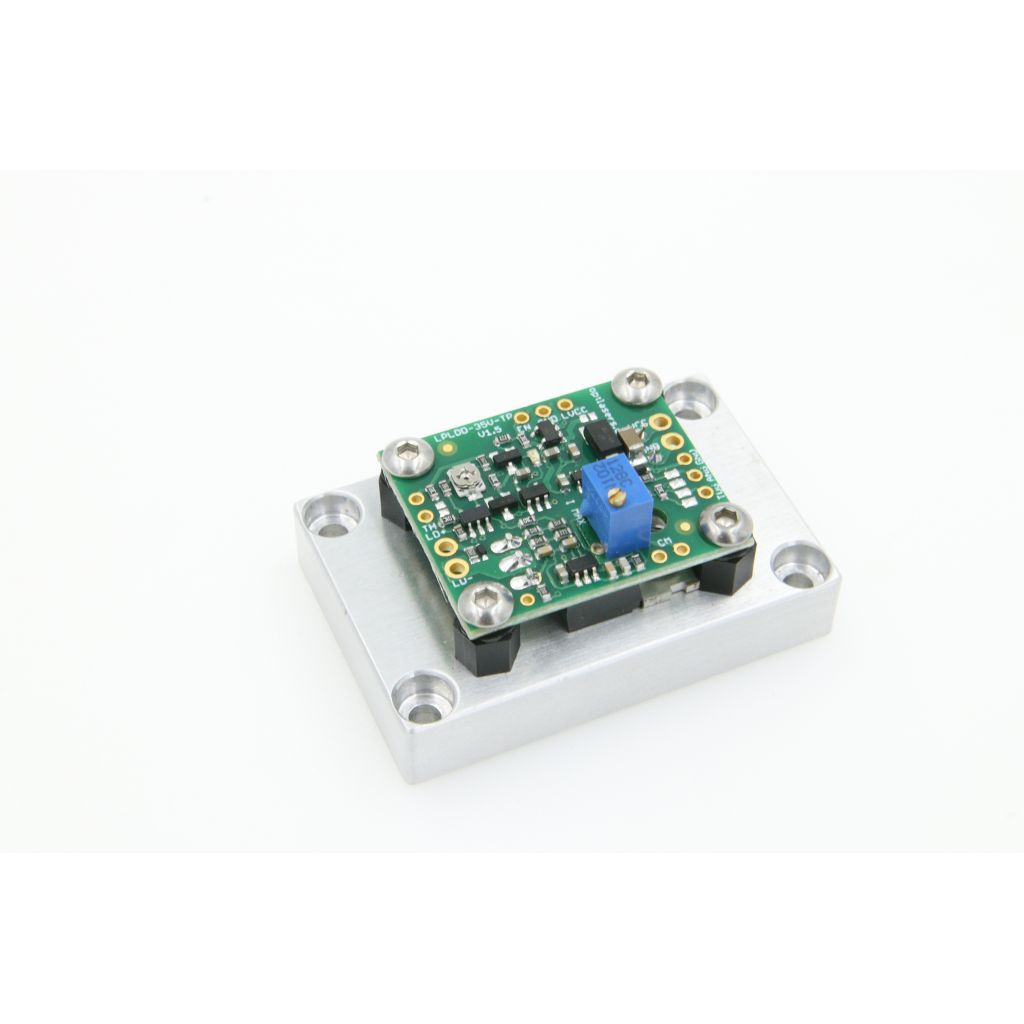
\includegraphics[scale=0.75]{98_images/ldd_optlaser.jpg}
    \caption{Der Diodentreiber von \textit{Opt Lasers} [21]}
    \label{fig:_diodentreiber_hw}
\end{figure}

Der Diodentreiber ist nach dem Schema angeschlossen, das in Abb. \ref{fig:diodentreiber_schema_hw} gezeigt ist. Der obere linke Block \textit{Control} beinhaltet das \textit{Toggle}-Signal, das analoge Signal und deren beiden Rückleiter. Die Energieversorgung darunter \textit{PSU 7.5-35V}, wird mit einem Gleichstrom mit 30V realisiert, dies ist weiter unten beschrieben. Auf der linken Seite mit \textit{LD} \textit{Light Diode}  bzw.  (dt. Leuchtdiode) beschriftet, ist der Ausgang an den die Pumpdiode angeschlossen wird. Abgebildet ist noch der \textit{Thermistor}, dieser soll die Temperatur der Diode überwachen und bei einer gewissen Temperatur den Ausgang entkoppeln und stromlos machen. Dies wurde in dieser Steuerung weggelassen, weil die Temperaturen der Diode und auch die des Gehäuses selber bereits überwacht werden. Dazu musste die Temperatursteuerung auf dem Diodentreiber überbrückt werden, auf dies wird hier jedoch nicht weiter eingegangen.

\begin{figure}[H]
    \centering
    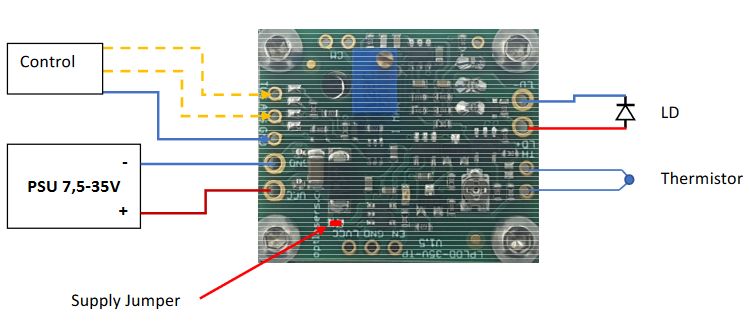
\includegraphics[scale=0.6, trim={0mm 0mm 0mm 0mm}, clip]{98_images/ldd_schema_connections.PNG}
    \caption{Das Schema des Diodentreibers von \textit{Opt Lasers}, wie dieser mit den anderen Komponenten der Steuerung verbunden ist. [21]}
    \label{fig:diodentreiber_schema_hw}
\end{figure}

Die in der Abb. \ref{fig:diodentreiber_modus_hw} gezeigte Darstellung ist das Signal zum Ansteuern des Diodentreibers. Die dunkel blaue (unterste) Linie, ist das Ausgangssignal, das direkt in die Pumpdiode eingespeist wird. Die grüne (mittlere) Linie, ist das Signal am analogen Eingang des Diodentreibers. Damit wird die Stromstärke am Ausgang gesteuert. Die orange (oberste) Linie ist das \textit{Toggle}-Signal, dies gibt die Ansteuerung frei, damit das analoge Signal zum Ausgang des Diodentreibers gelangt. [21]

\begin{figure}[H]
    \centering
    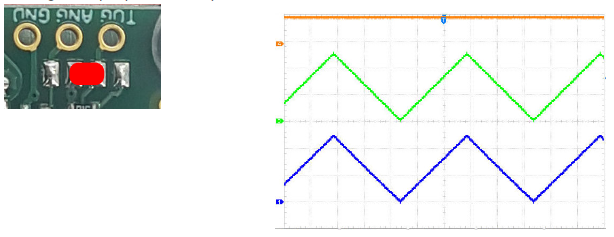
\includegraphics[scale=0.75, trim={70mm 0mm 0mm 0mm}, clip]{98_images/ldd_schema_modus.PNG}
    \caption{Die Steuerungssignale für den Diodentreiber von \textit{Opt Lasers}. Die Markierungen am linken Rand sind jeweils die Nullstellen der Signale. [21]}
    \label{fig:diodentreiber_modus_hw}
\end{figure}

Die Logik der Steuerung ist in Tab. \ref{fig:diodentreiber_modus_hw} gezeigt. Diese Konfiguration wurde aus einer Palette von möglichen Konfigurationen ausgewählt. Sie erfüllt alle Kriterien, die der Diodentreiber innehaben muss, um die geforderten Aufgaben zu leisten.

\begin{table}[H]
    \centering
    \begin{tabular}{c|c|c}
         Analogsignal&       \textit{Toggle}-Signal&     Ausgang\\
         \hline
         0&             0&          0\\
         0&             1&          0\\
         1&             0&          0\\
         1&             1&          1
    \end{tabular}
    \caption{Die Wertetabelle der Ansteuerung des Diodentreibers.}
    \label{tab:ldd_wertetabelle}
\end{table}

\subsection{Energieversorgung}
Die benötigte Leistung des Netzteils für das gesamte System beläuft sich auf etwa 80W. Dies wurde einerseits errechnet (s. Anhang \ref{formula:_calculation_sp_power}), andererseits mit einem digitalen Netzteil, an dem alle Komponenten bis auf den Diodentreiber angeschlossen wurden, verifiziert. Die elektrische Leistung des Diodentreibers beträgt maximal 52.5W, was das die Leistung des Netzteils noch nicht erschöpfen würde.\\
\begin{equation}
P_{EL.GES} = 2*P_{TEC}+P_{RPI}+P_{LDD}+P_{VENT} = 2*8W+12W+52.5W+1.06W \approx 87.5W
    \label{formula:_calculation_sp_power}
\end{equation}

Die Pumpdiode wird mit 30V gespiesen, wohingegen der Rest der Steuerung mit 24V betrieben wird. Dies verlangte, dass entweder zwei Netzteile eingesetzt wurden oder aber ein Netzteil und ein DC/DC-Wandler, der die Spannung des Netzteils auf die benötigten 24V transformiert, zum Einsatz kommt. Die Entscheidung fiel auf die Version mit dem DC/DC-Wandler. Dieser ist im Volumen massiv kleiner und nimmt somit weniger Platz im Gehäuse in Anspruch. Dieser kann eine Spannung von bis zu 36V aufnehmen und misst 24V beim Ausgang. Wie weiter oben erwähnt, kann der DC/DC-Wandler eine maximale Leistung von 30W ausgeben. Diese Leistungsgrenze wird in vollem Betrieb der Steuerung ausgeschöpft. Die Leistungsbezugsgrenze wurde wie oben erwähnt, in den Leistungsbezüger limitiert.

\begin{figure}[H]
%https://www.reichelt.com/ch/de/schaltnetzteil-geschlossen-195-w-36-v-5-5-a-mw-rsp-200-36-p147907.html?PROVID=2808&gad_source=1&gclid=Cj0KCQiA5-uuBhDzARIsAAa21T-__vZqX_esib7CfoGVmrPyoBO7UXEfQpRHOOkOo2j1YGIXCt2oLD0aAhbVEALw_wcB
    \centering
    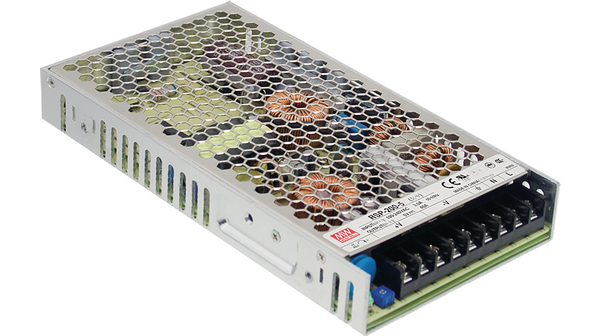
\includegraphics[scale=0.35]{98_images/schaltnetzteile-200-w-pfc.jpg}
    \caption{Das Netzteil des Herstellers \textit{Mean Well}. [9]}
    \label{fig:controller_ps_hw}
\end{figure}

\begin{figure}[H]
% https://www.conrad.ch/de/p/mean-well-rsd-30g-24-dc-dc-wandler-12-v-dc-24-v-dc-36-v-dc-24-v-dc-1-25-a-30-w-1761269.html?gclid=CjwKCAiA6KWvBhAREiwAFPZM7vuk7TGgJgOWfGuP3-sRh1IH8ajzLsO8kXYmecqB9bC_QCBB2CDiuhoC8NAQAvD_BwE&utm_source=google-shopping-de&utm_medium=search&utm_campaign=shopping-online-de&utm_content=shopping-ad_cpc&WT.srch=1&ef_id=CjwKCAiA6KWvBhAREiwAFPZM7vuk7TGgJgOWfGuP3-sRh1IH8ajzLsO8kXYmecqB9bC_QCBB2CDiuhoC8NAQAvD_BwE%3AG%3As&gad_source=1
    \centering
    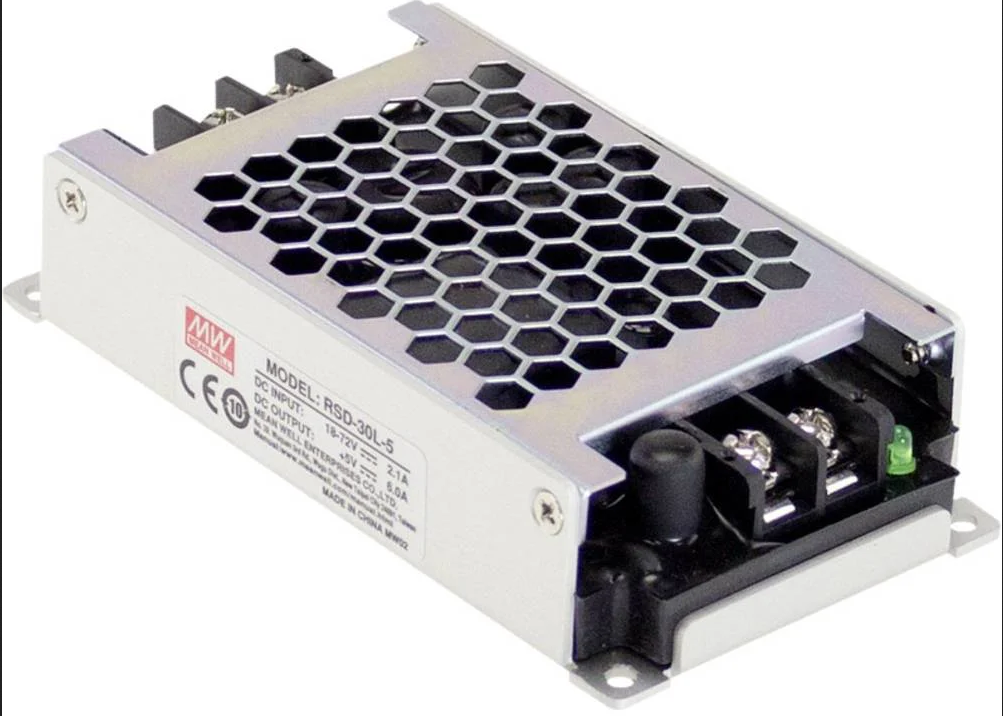
\includegraphics[scale=0.2, trim={2mm 2mm 2mm 2mm}, clip]{98_images/mean_well_dc_dc_converter.PNG}  
    \caption{Der eingesetzte DC/DC-Wandler, des Herstellers \textit{Mean Well}. [9]}
    \label{fig:dc_dc_wandler_hw}
\end{figure}

\subsection{Sensorik}
Die Positionen der Temperaturmessung des Alexandritkristalls ist in der Abb.\ref{fig:temp_measurement_hw_1} dargestellt. An diesen Positionen stört sie den Laser im Betrieb nicht und die Temperatur kann trotzdem möglichst nahe an der Quelle messen werden. Die Temperatur für den Kristall soll sich im Bereich von 20°C befinden, bei der Pumpdiode bei etwa 18°C. Thermoelektrische Kühler der Art, die in der Abb. \ref{fig:tec_controller_free} sind jeweils eingebaut. Für die Messung der Temperatur des Kristalls wird ein NTC 10k$\Omega$, $\beta$=3950 Thermistor verwendet. Der Typ des Thermistors der Pumpdiode konnte nicht herausgefunden werden. Die Parameter des Thermistors müssen mit Messungen ermittelt werden.\\

In der Abb. \ref{fig:temp_measurement_hw_1} ist die Pumpdiode gezeigt. Diese hat bereits einen integrierten Temperatursensor, der direkt angeschlossen werden kann.

\begin{figure}[H]
    \centering
    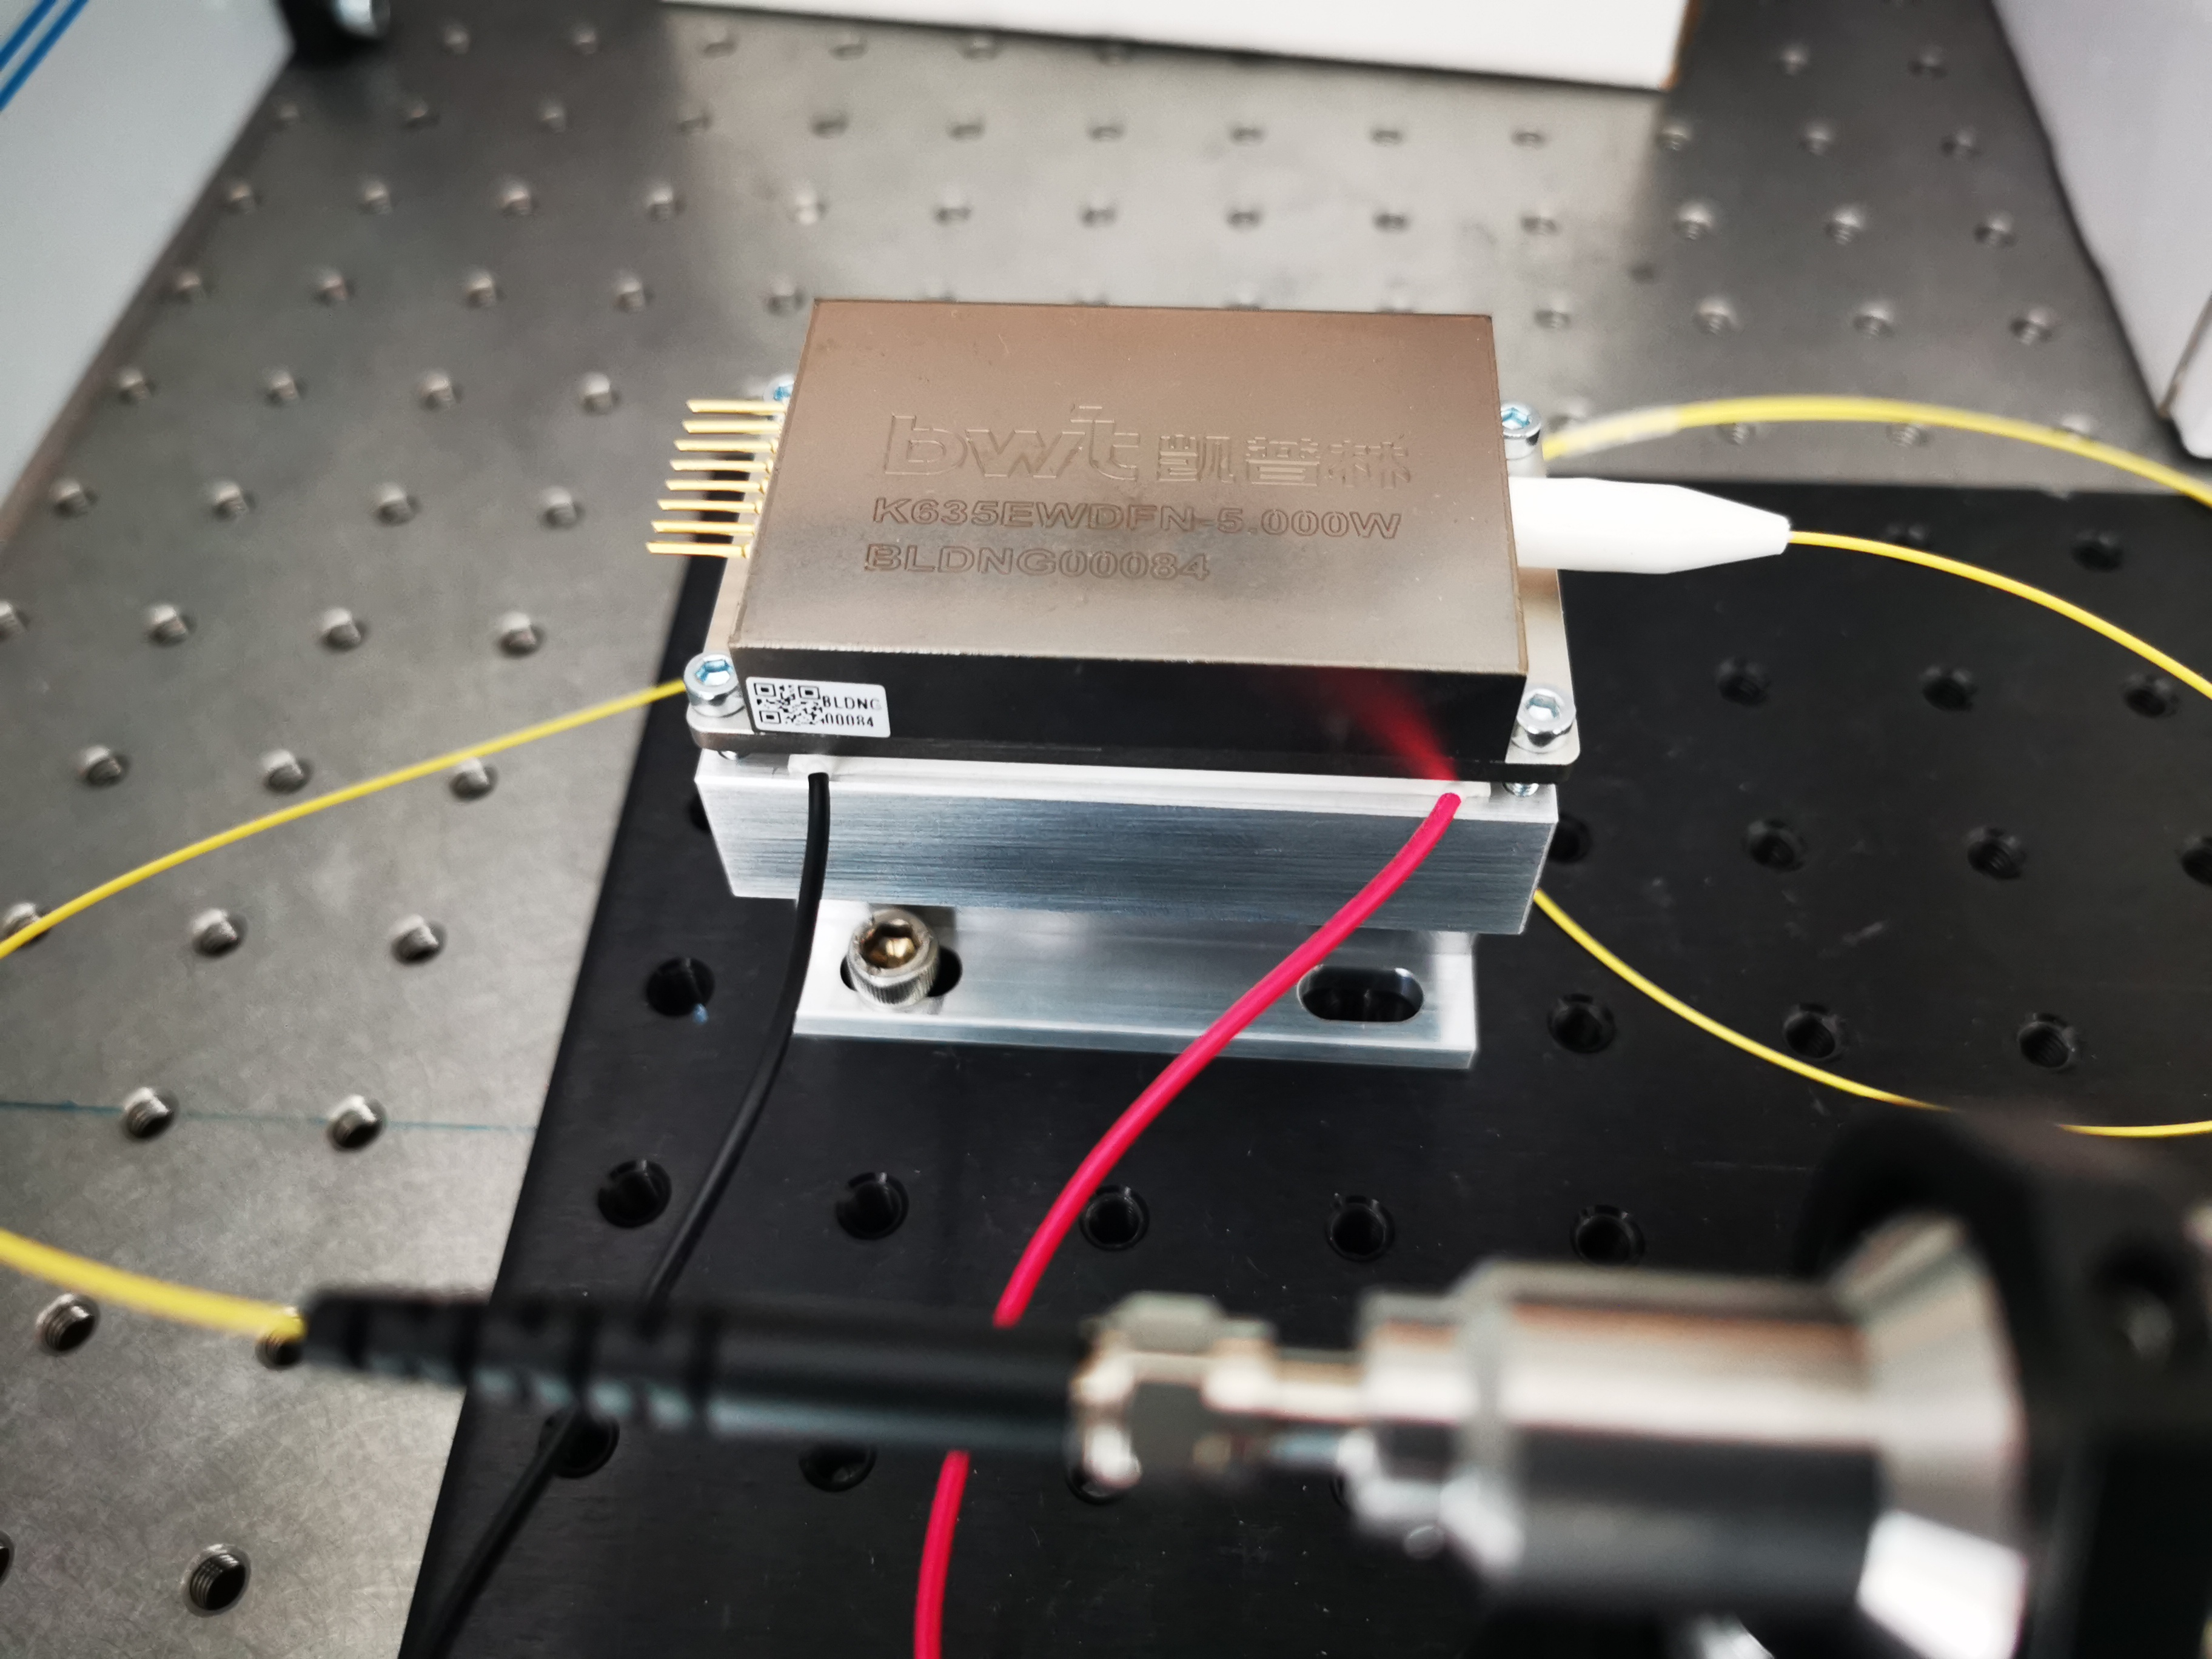
\includegraphics[scale=0.08, trim={300mm 300mm 200mm 150mm}, clip]{98_images/IMG_20240322_111841.jpg}
    \caption{Positionen des Temperaturfühler der Pumpdiode.}
    \label{fig:temp_measurement_hw_1}
\end{figure}

Der Thermistor der Pumpdiode ist an Pin 5 und 6 anzuschliessen. Ersichtlich in Tabelle \ref{tab:_pump_pins}.

\begin{table}[H]
    \centering
    \begin{tabular}{l|c|l}
         \textbf{Schema}&     \textbf{Pin}&      \textbf{Funktion}\\
         \hline
         \multirow{8}{*}{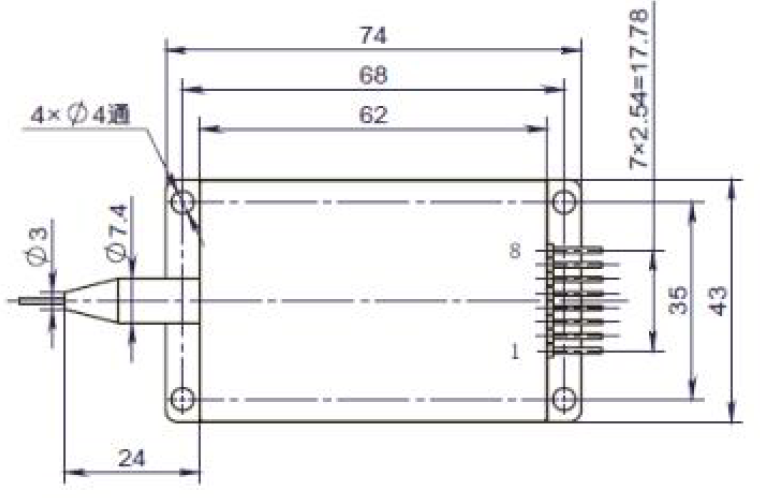
\includegraphics[scale=0.6]{98_images/pumpdiode_pins.PNG}}&8&LD (-)\\
         &                  7&                          None\\
         &                  6&                          Thermistor\\
         &                  5&                          Thermistor\\
         &                  4&                          PD (P)\\
         &                  3&                          PD (N)\\
         &                  2&                          None\\
         &                  1&                          LD (+)\\
    \end{tabular}
    \caption{Die Pin-Belegung der Pumpdiode. (Beachte Reihenfolge Pins) [25]}
    \label{tab:_pump_pins}
\end{table}

Beim Kristall in Abb. \ref{fig:_thermistor_cr}, soll der Thermistor an gezeigter Stelle platziert werden.

\begin{figure}[H]
    \centering
    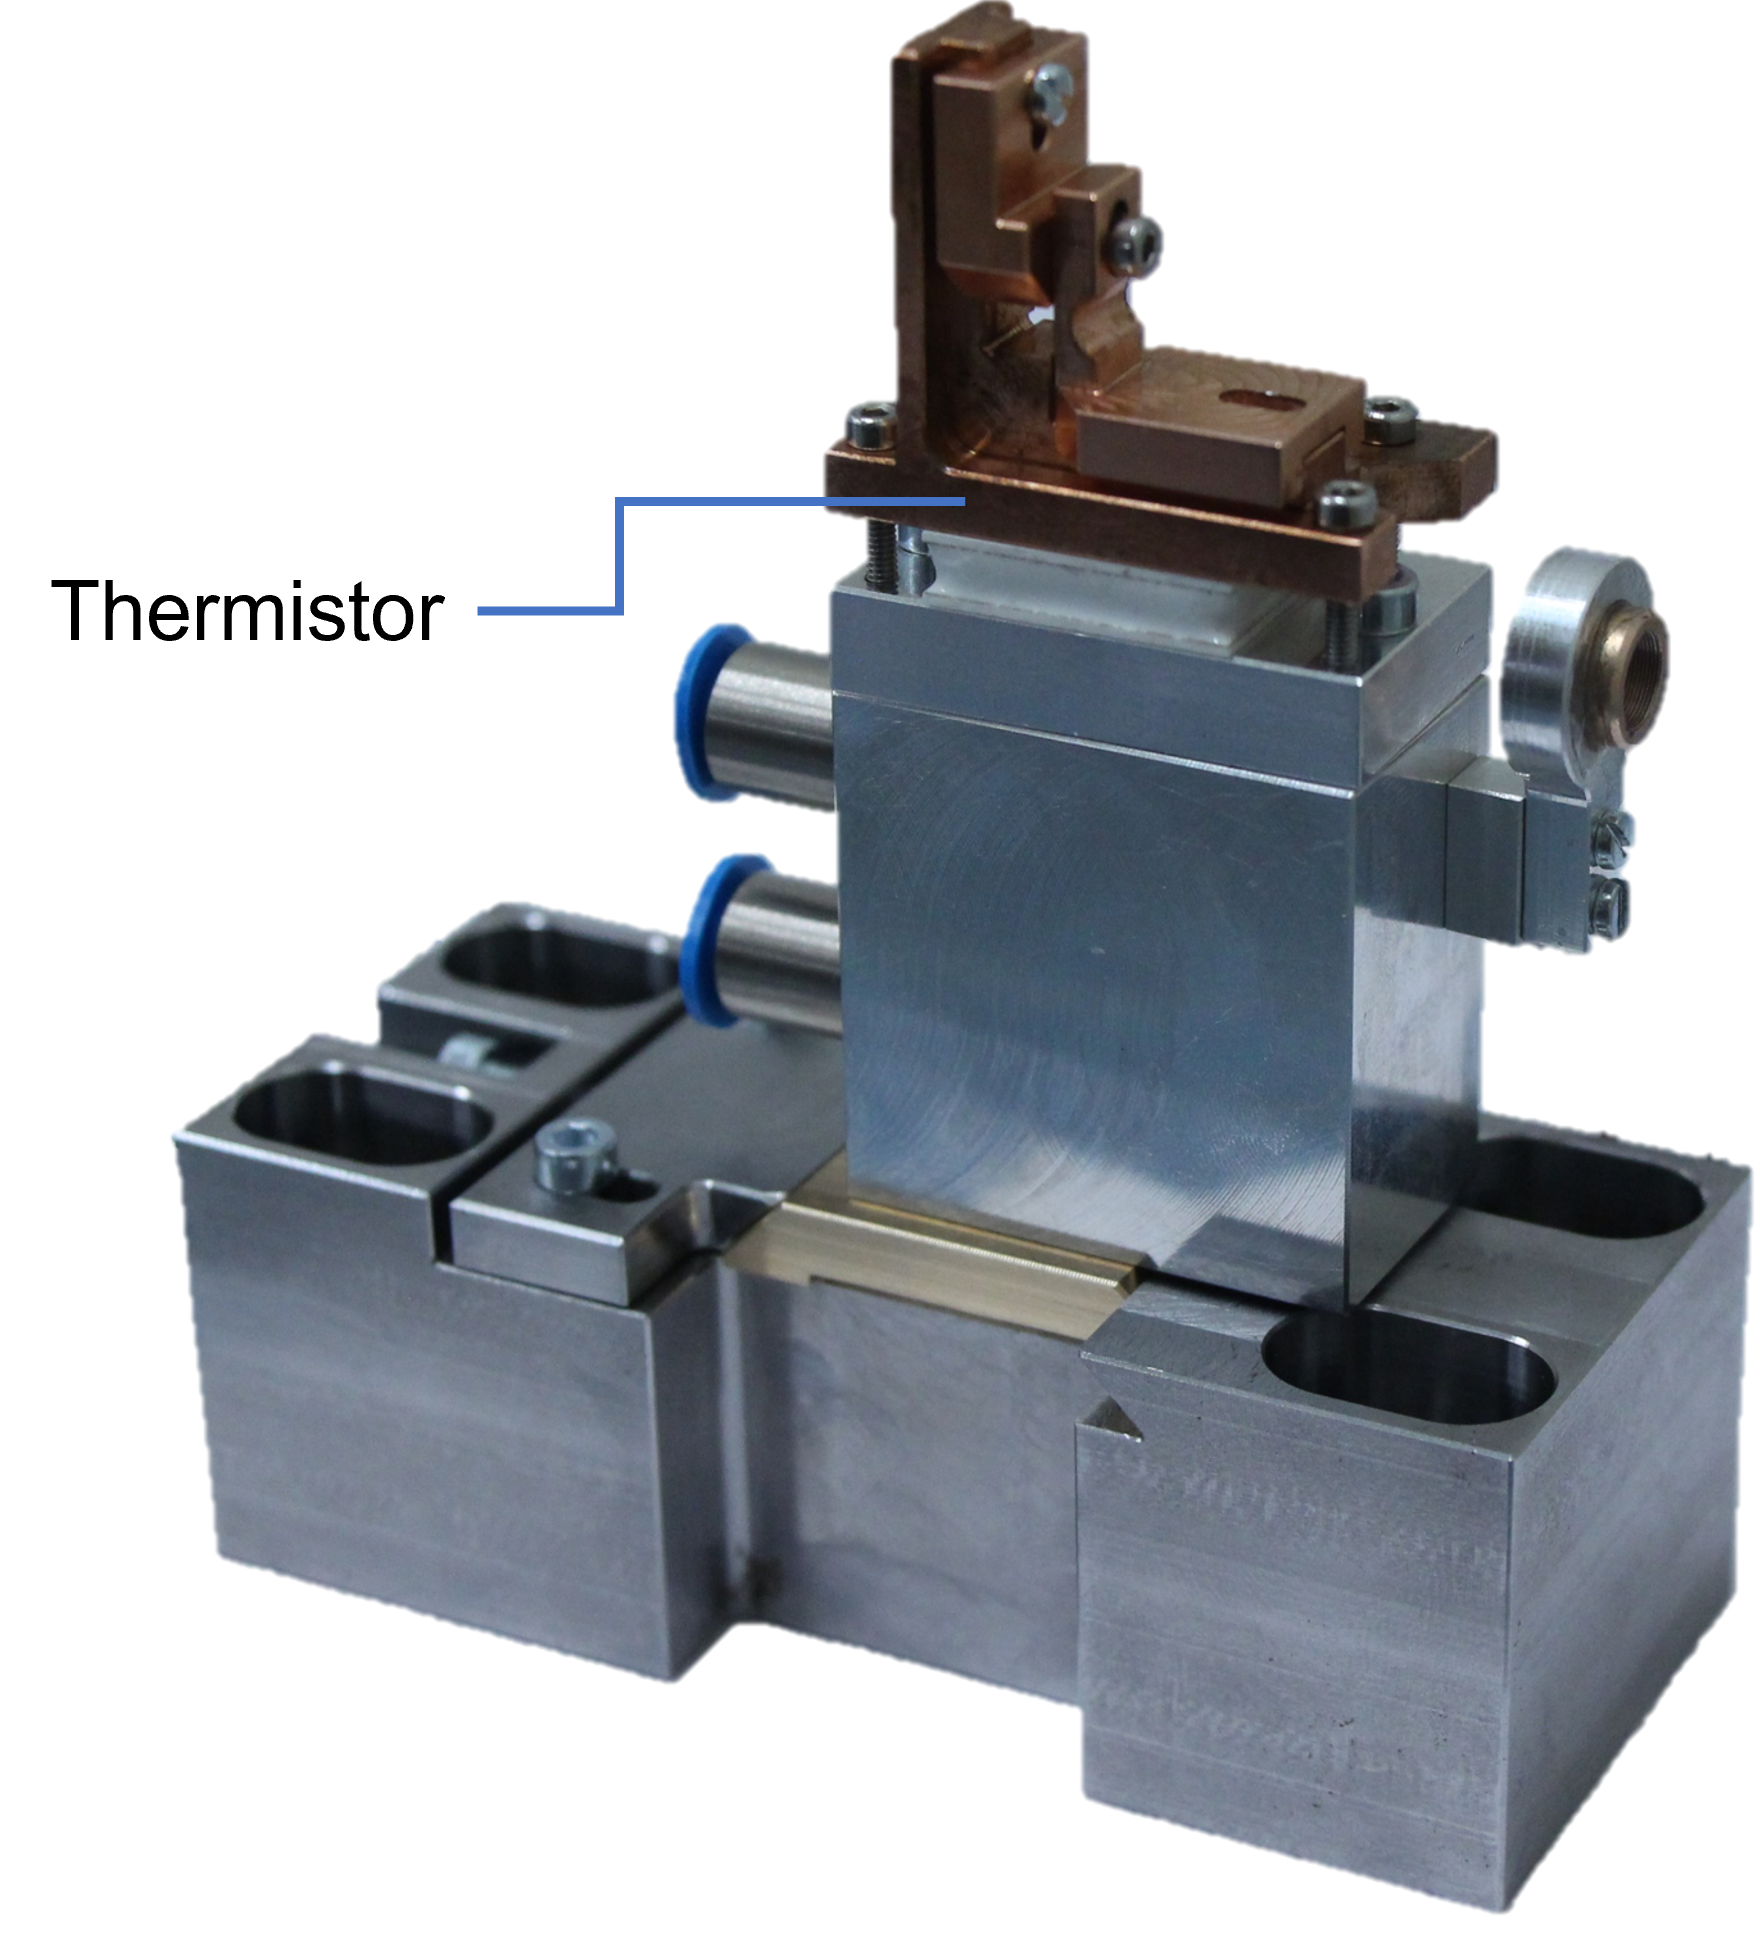
\includegraphics[scale=0.5, trim=0mm 70mm 0mm 0mm, clip]{98_images/thermistor_cr.png}
    \caption{Die Position des Thermistors für den Kristall.}
    \label{fig:_thermistor_cr}
\end{figure}

\subsection{Digitalanzeige}
Für die Digitalanzeige waren vor allem drei Aspekte ausschlaggebend, um die gewünschte Funktion zu gewährleisten. Die Eingabe der Werte, die Anzeige der Werte und die Verständlichkeit der angezeigten Werte. All die Kriterien sollten erfüllt werden, um die Steuerung des Lasers optimal zu gewährleisten. In der folgenden Tabelle wurden einige Kriterien die die zuvor genannten Aspekte ermöglichen sollen aufgelistet. Auch aus Sicherheitsgründen muss die Ergonomie der Anzeige intuitiv gestaltet sein und muss im Notfall beherrschbar bleiben. Es werden zwei Displaytypen einander gegenüber gestellt, damit der optimalen Displaytyp evaluiert werden kann.

\begin{table}[H]
    \centering
    \begin{tabular}{l|l|l}
        \multicolumn{1}{c|}{$-$}&        \textbf{16x2 mit Taster}&       \textbf{800x480 Touchanzeige}\\
        \hline
        Bedienung&                      $-$ Taster Analogeingänge&      $+$ Touch integriert\\
        Anzeige&                        $-$ Kleine Anzeige&             $+$ Grössere Anzeige\\
        Verständlichkeit&               $-$ Kryptische Anzeige&         $+$ Verständliche Anzeige\\
        Benutzerführung&                $-$ Tieferes Menü&              $+$ Weniger tiefes Menü\\
        Programmierung&                 $+$ Einfache Programmierung&    $-$ Anspruchsvolle Programmierung
    \end{tabular}
    \caption{Pro - Kontra Liste für die Auswahl der Digitalanzeige}
    \label{tab:choice_display_hw}
\end{table}

Die Entscheidung fiel auf die Touch-Anzeige. Zusätzlich lassen sich alle Komponente wie Knöpfe direkt in die Anzeige programmieren. Es müssen keine komplexen Abläufe programmiert werden, die die Betätigung sogenannte \textit{interrupts} der physischen Knöpfe erkennt und das Programm lenkt. [5] Zusätzlich müssen keine Ein-/Ausgänge zusätzlich auf der SPS einprogrammiert werden. Mit der Anzeige können ganze Designs erstellt werden, was das Arbeiten mit der Steuerung ergonomischer macht.

\subsection{Testaufbau - Mock-up}
In einem Mock-up aus Karton mit den gleichen Dimensionen, wie das finale Steuerungsgehäuse, konnten die Funktionen und das Verhalten der Steuerung geprüft werden. Darunter wurde getestet, ob die Temperaturen in der Steuerung in einem gewünschten Rahmen von 40°C - 65°C blieben. $[7]$ Gemessen werden die Temperaturen mit der internen Temperaturmessung des Prozessors des Raspberry PI. Ergänzend wurden die Positionen der Komponenten im Gehäuse wurde mit Hilfe von CAD-Software geprüft. Danach wurden die oben genannten Bleche erstellt und die Komponente mit Verschraubungen platziert. Für die Bleche hatte das bestehende Gehäuse bereits Verschraubungen, die verwendet werden konnten. Das CAD-Modell des Gehäuses mit den Komponenten sind im Anhang im Kapitel \ref{chptr:_cad_gehäuse} aus verschiedenen Perspektiven gezeigt.

\subsection{Konstruktion des Gehäuses}
Wie im vorherigen Kapitel angedeutet, war das Gehäuse bereits vorhanden. Die oben aufgelisteten Komponenten wurden auf zusätzlichen Blechen montiert, in die Gewindelöcher eingebracht wurden. Durch die konvexe Form der Seiten des Gehäuses entstand im Inneren des Kontrollers auf diesen Blechen mehr Fläche für die Komponenten. Dies vereinfachte die Montage. Zusätzlich mussten noch die Zugänge für die Verkabelung der Stromversorgung, deren Schalter und das Kabel für die Ansteuerung der Komponenten im Laser-Aufbau angepasst werden. Dafür wurden sämtliche Löcher für spätere Erweiterungen beibehalten. Auf der Abb. \ref{fig:controller_free} ist die Front des Kontrollers zu sehen, in der Mitte die Touch-Anzeige für die Bedienung der Steuerung. Alle oben genannten Komponenten befinden sich in der Steuerung.

\begin{figure}[H]
    \centering
    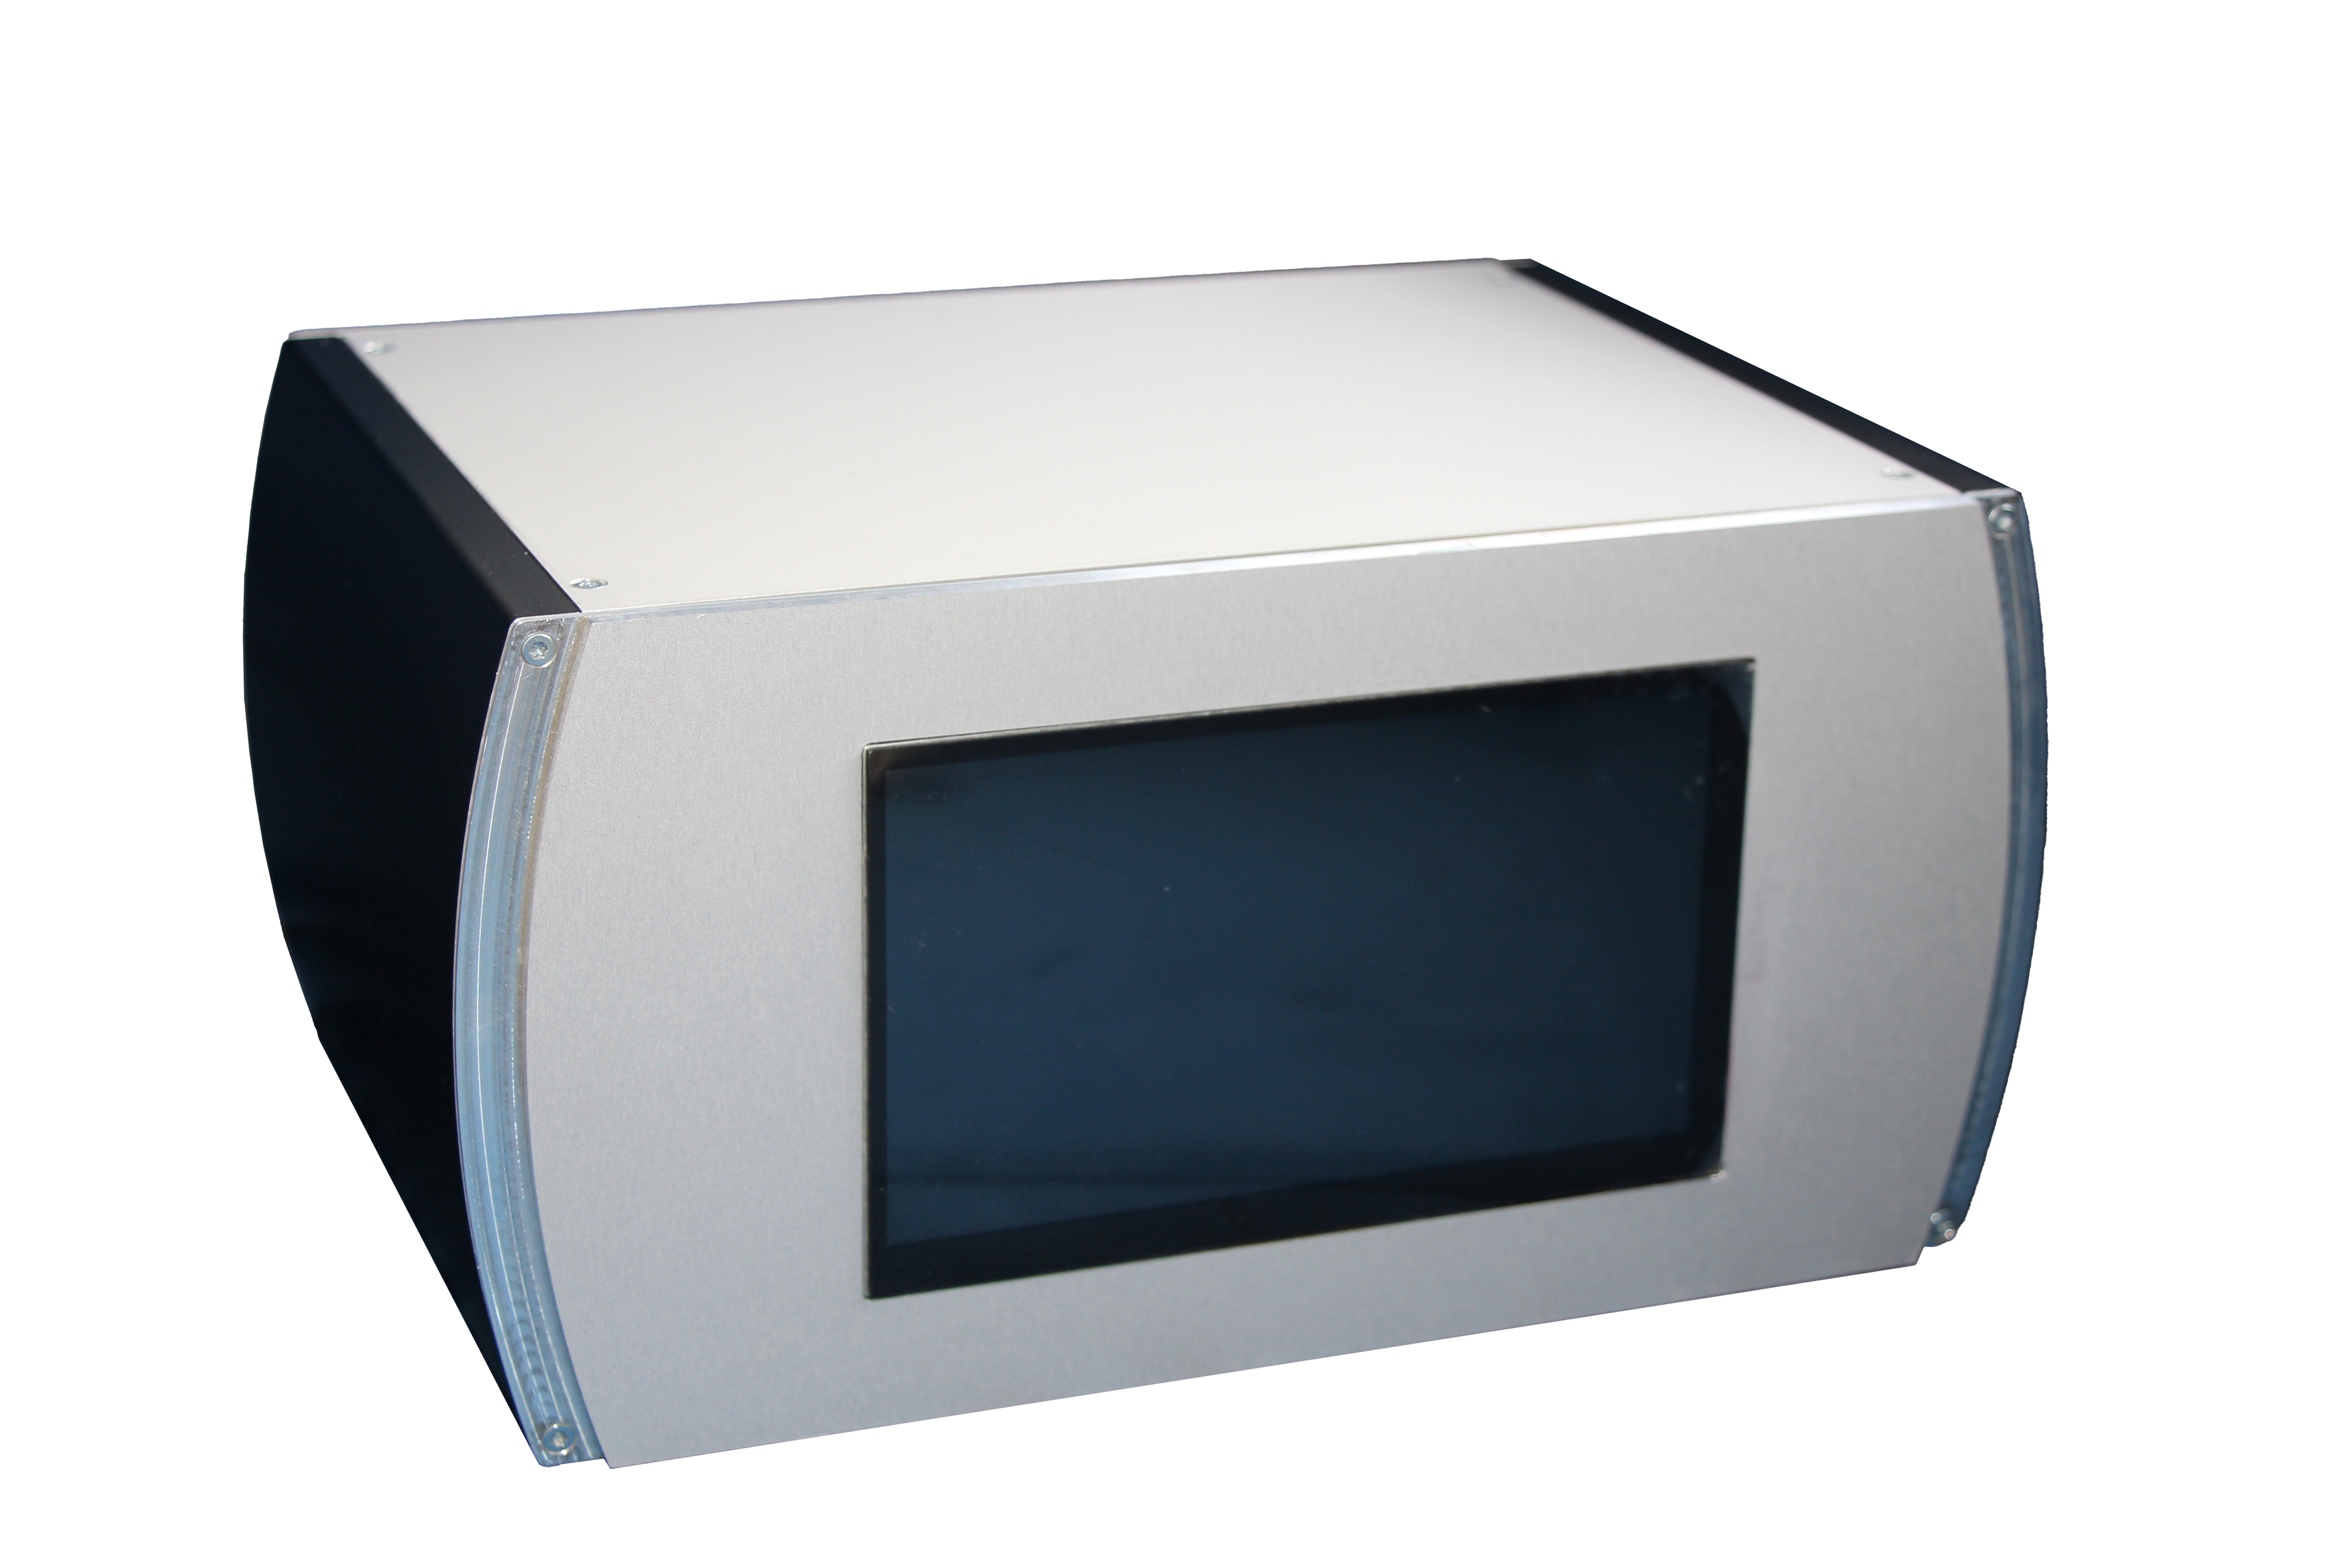
\includegraphics[scale=0.08]{98_images/IMG_6193_freigestellt.png}
    \caption{Front der abgeschlossenen Steuerung.}
    \label{fig:controller_free}
\end{figure}

\begin{figure}[H]
    \centering
    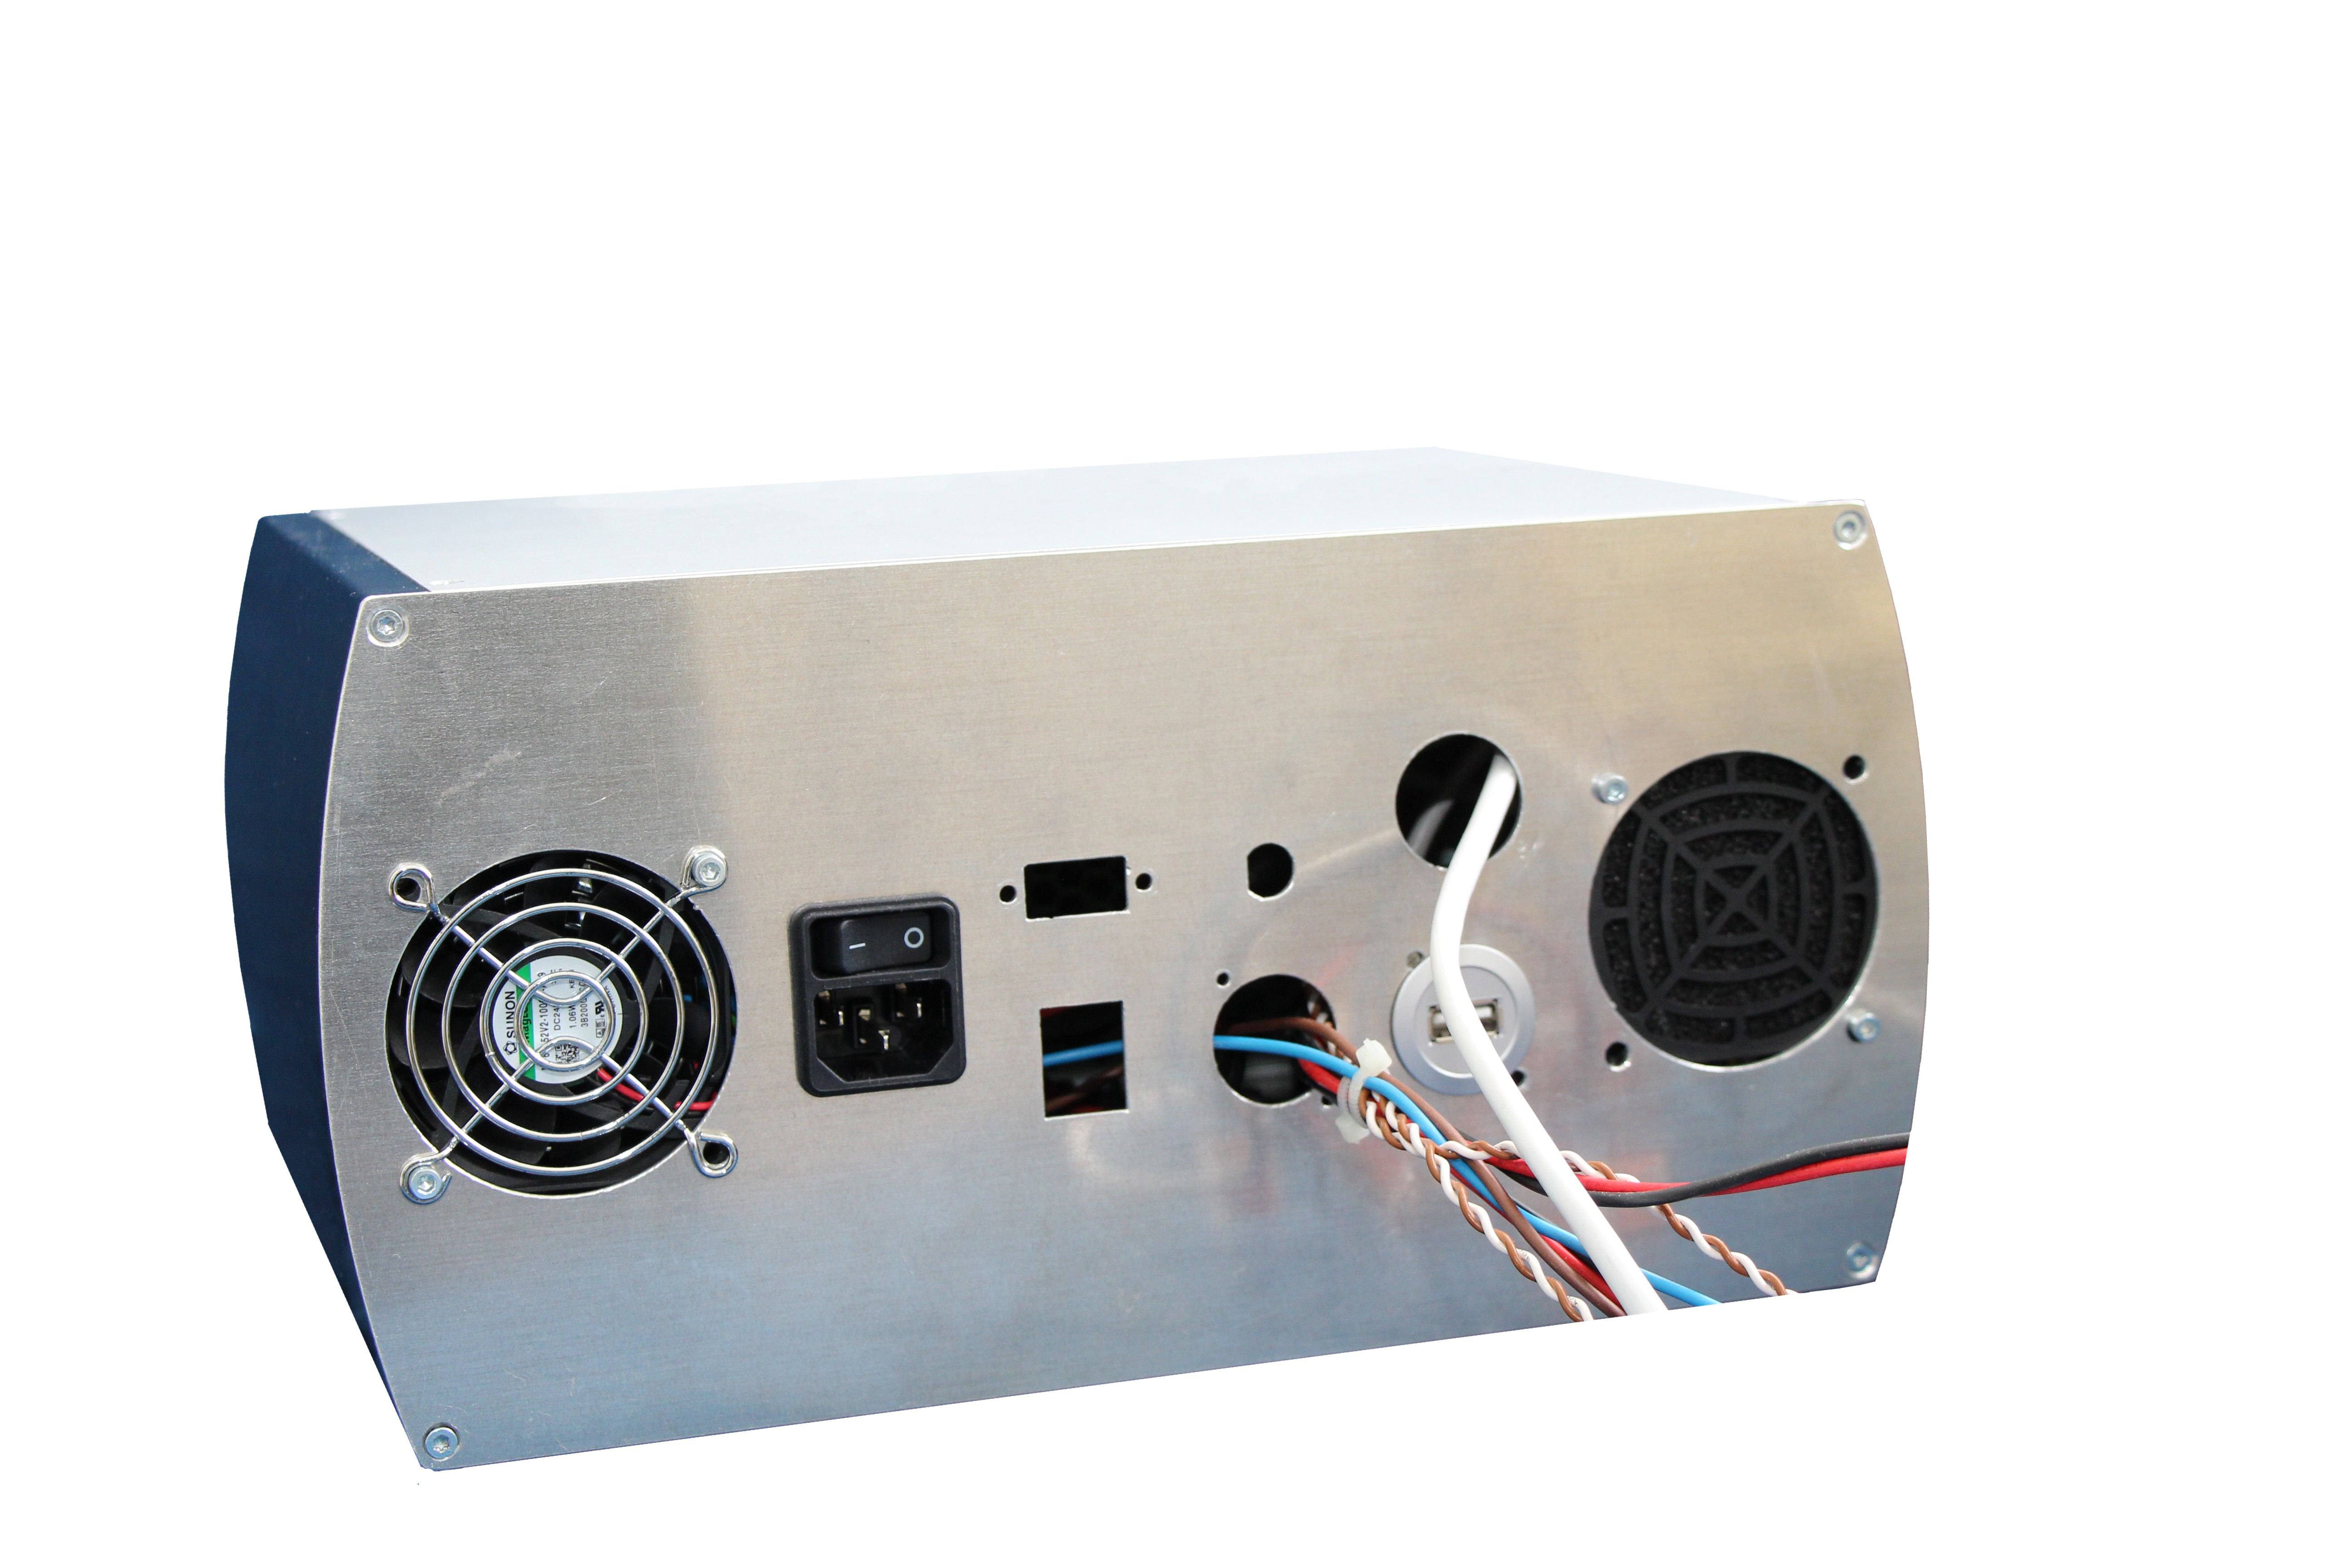
\includegraphics[scale=0.08]{98_images/controller_box_back.png}
    \caption{Rückseite der abgeschlossenen Steuerung.}
    \label{fig:controller_free}
\end{figure}

\clearpage